%% The following is a directive for TeXShop to indicate the main file
%%!TEX root = diss.tex

\chapter{A Description of 3D Reconstruction}
\label{ch:3DRecon_Desc}
In Chapter~\ref{ch:3DRecon_Taxo}, we introduce a taxonomy of 3D reconstruction which maps algorithms according to the visual/geometric characteristics of the object. However, without a formal `language', \ie a model and representations, the mapping from an algorithm to a volumn of the problem space would be largely empirical. Without a formal definition of the problem space, expressing the condition that an algorithm works well is not a well defined problem.

Computer vision problems require, among other factors, a model of the problem domain~\cite{little1985phdthesis}. The relevant properties of the elements in the domain must be characterized and their relations must be analyzed. Representations describe the object properties selected by the model to facilitate solution of the problem. For instance, surface orientation is a geometric model, and surface normal or curvature are representations of this mdoel. More specifically in the case of reconstruction problem, we first need to establish a model that defines the problem domain, then properties of the objects and surfaces are investigated to see their influence on the problem domain, which serves as the representation of the reconstruction problem.

In this chapter, we attempt to extend this taxonomy by providing a description of 3D reconstruction problem which allows for a well defined specification of the visual cues surrounding the problem and of the range of the desired solution, abstracting away from the functional specification of \textit{how} to estimate a reconstruction. We first propose a formal definition of the 3D reconstruction problem in Section~\ref{sec:3DRecon_Def}. Section~\ref{sec:3DRecon_Model} discusses various key \textit{aspects} of the problem space that are crutial to describe the appearance of the object. Section~\ref{sec:3DRecon_Rep} the actual concrete representations of the proposed model. Section~\ref{sec:3DRecon_Exp} provides examples of expressing common 3D reconstruction problems using the proposed model and representations. These four layers: Definition, Representation, Model, and Expression represent out framework of accessible 3D reconstruction.

\section{Definition}
\label{sec:3DRecon_Def}
We first give the definitions of some basic concepts, which include general computer vision concepts such as scene, camera, and image. We then define some other notions that are close related to the reconstruction problem before a formal definition is introduced. We then provide some reasonable approximations for a more practical definition.

\subsection{Basic notations}
We use the following notations: $\{C_n\}_{n=0}^{N-1}$ represents the camera set, which include both the intrinsic and extrinsic parameters; $\{I_n\}_{n=0}^{N-1}$ represents the set of all images; $\{L_n\}_{n=0}^{N-1}$ represents the set of light sources.

\textbf{Definition 1 (Scene)} The scene $S$ is the four-dimensional joint spatio-temporal target of interest.

\textbf{Definition 2 (Image)} The 2D observation of the 3D scene $S$ on the image plane of camera $C_i$ at time $t_0$, which is modelled as: $I_i = T(S, C_i, L_0, t_0)$, or on the image plane of $C_0$  under the light source $L_i$ at time $t_i$, $I_i= T(S, C_0, L_i, t_i)$, where $T$ is the geometric/radiometric transformation.

The transformation $T$ can be a geometric one which determines the 2D coordinates of a 3D point, or a radiometric one which determines the intensity/irradiance information from the information of illumination, viewing direction and surface orientation, or both.

\subsection{Segment and Scell}
\textbf{Definition 3 (Segment)} A segment is a distinct region in the image.

Segment is the most basic element in the image, can be considered as a generalized pixel. For instance, a segment can be a pixel, a window area, an edge, a contour, or a region of arbitrary size and shape.

\textbf{Definition 4 (Cue)} cues are the visual or geometric characteristics of the segments $seg$ that can be used for reconstruction, denoted as $cue(seg)$.

For instance, the cue can be texture within a window area, intensity/colour value of a pixel, or object contour, etc.

\textbf{Definition (scell)} A Scell (scene element) is a volume in the scene which corresponds to at least one segment.

A scell can be considered as a generalization of a voxel. However, a scell is not necessarily distinct since

\textbf{Definition (Property)} Properties are the visual and geometric characteristics of the Scell $sc$, which would influence the cues of a segment, denoted as $prop(sc)$.

The property of the scell can be the 3D position or orientation information, visual texture, reflectance, surface orientation, roughness, convacity, etc.

The relation between the notions define above is shown in Figure~\ref{seg_scell}.
\begin{figure}[h]
\centering
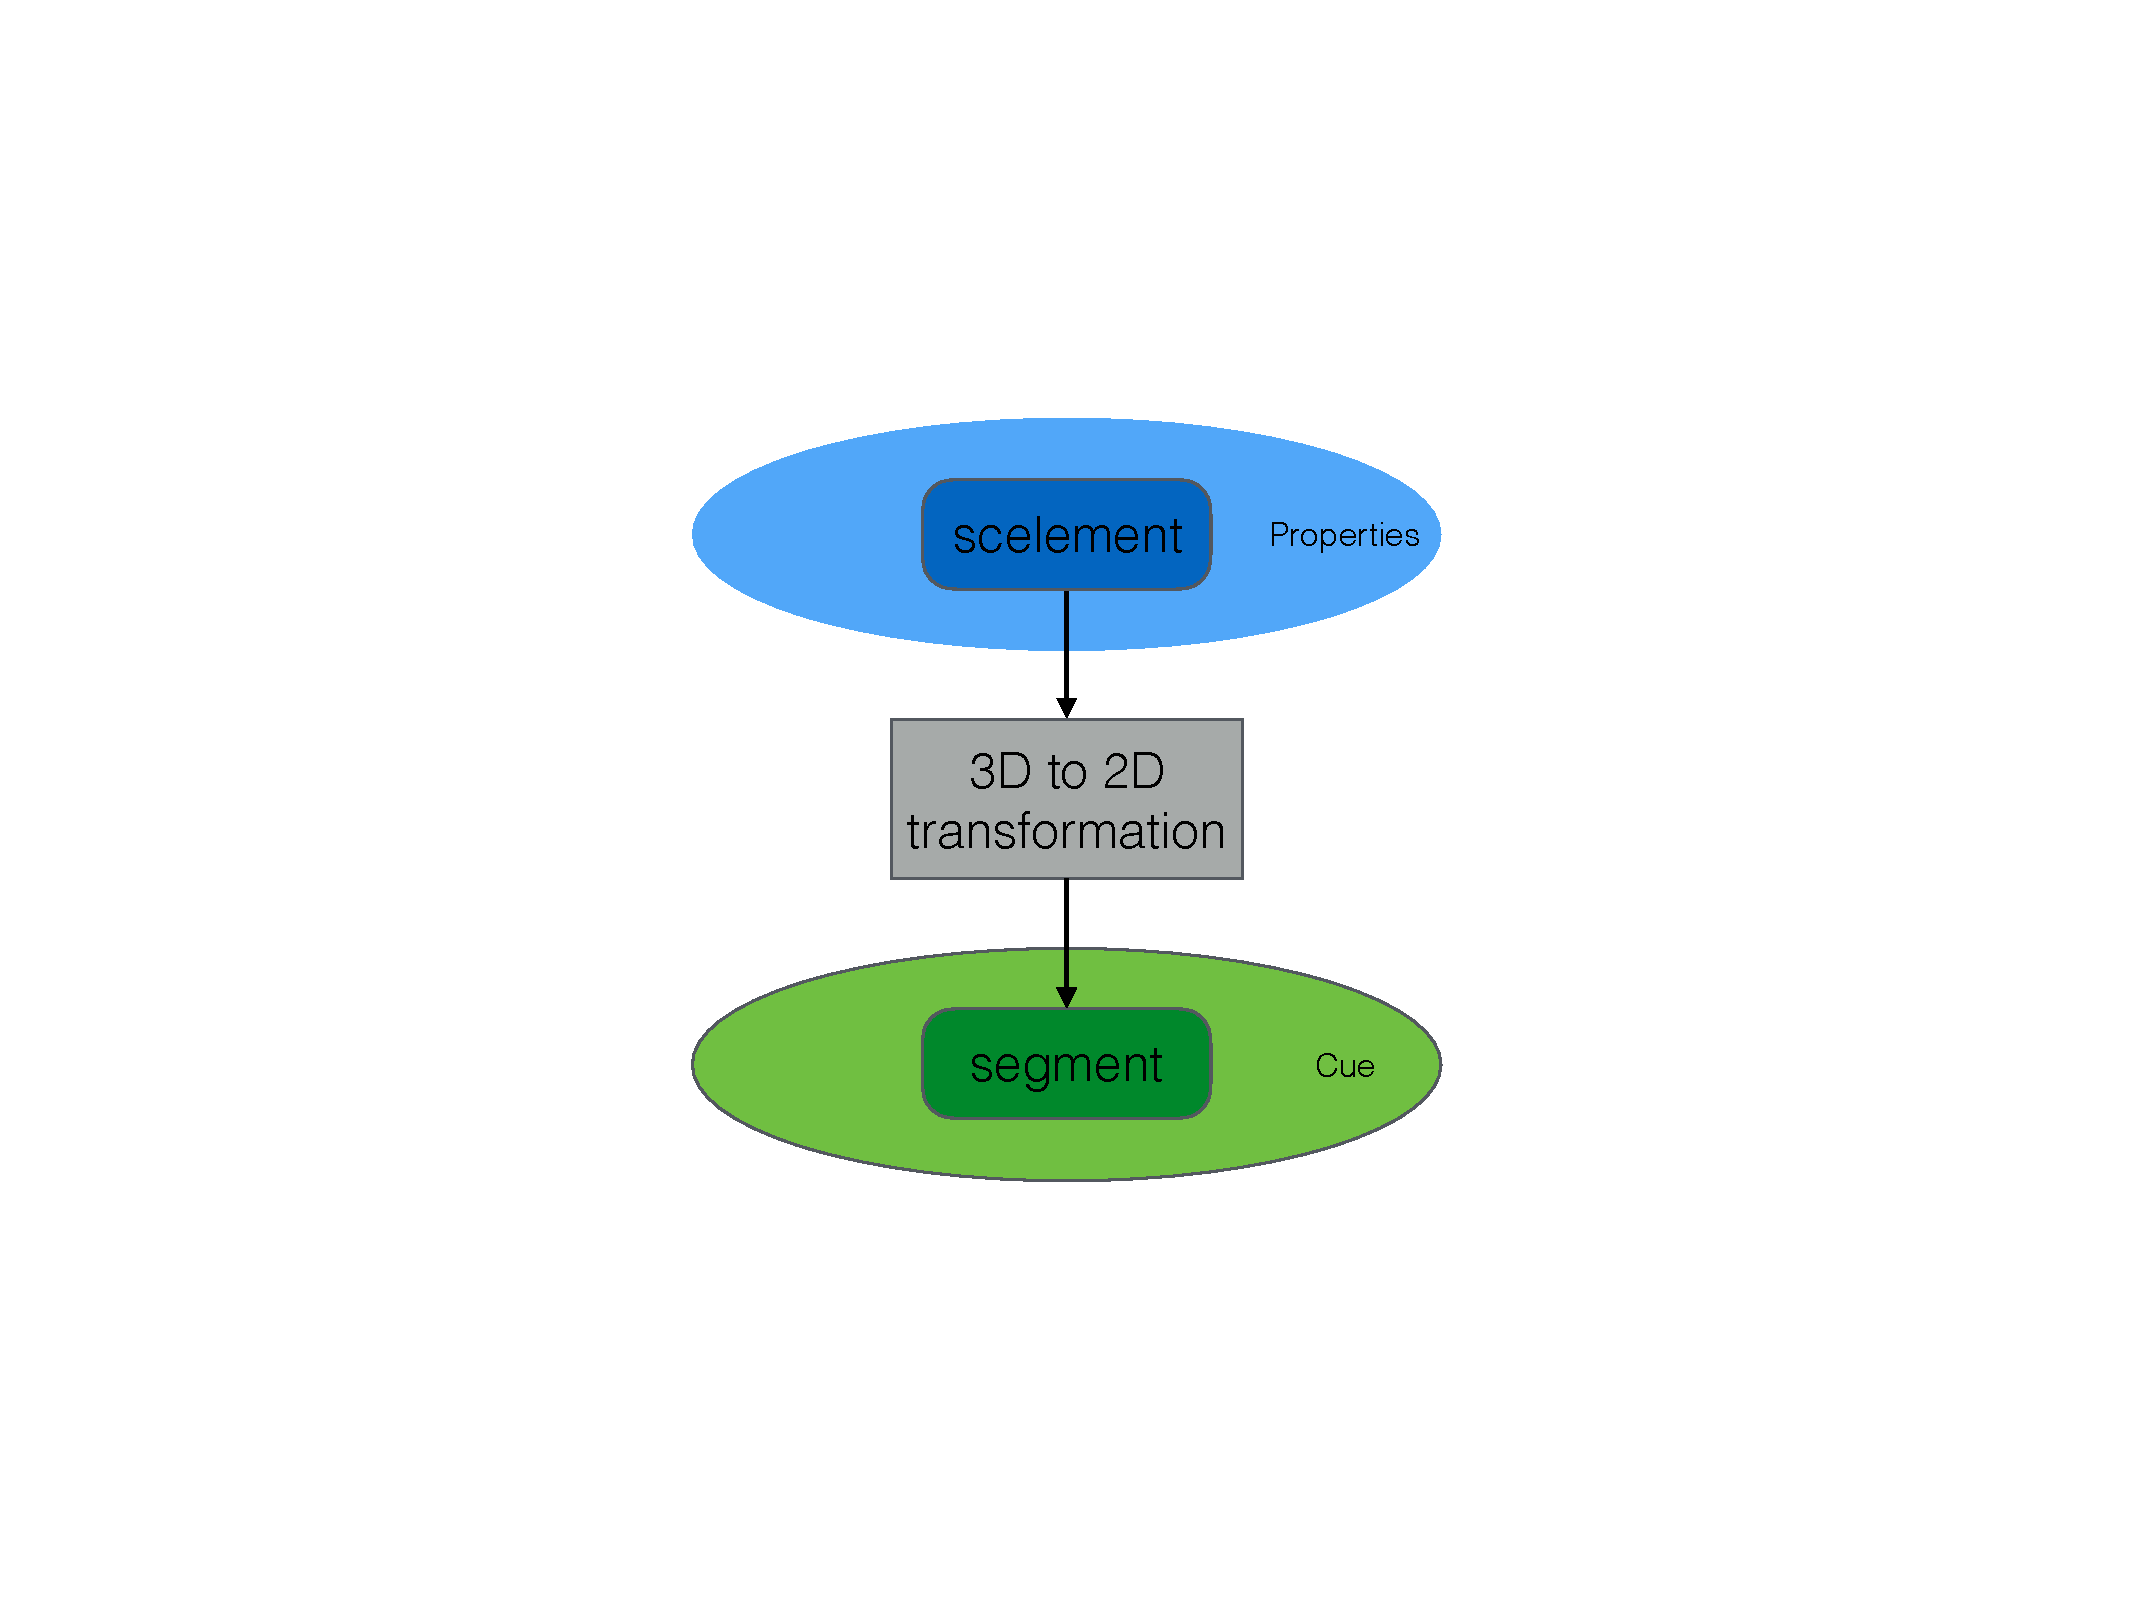
\includegraphics[width=0.5\textwidth]{model/seg_scell}
\caption{Relation between a scell and a segment}
\end{figure}

% \textbf{Definition (Representation)} The scell can be represented as a voxel, a depth value, a 3D point/patch, or a surface normal, etc, which is denoted as $rep(sc)$.

\subsection{Photo-consistency}
Every photograph of a 3D scene taken from a camera $C_i$ partitions the set of all possible shape-radiance scene descriptions into two families, those that reproduce the photograph and those that do not. We characterize this constraint for a given shape and a given radiance assignment by the notion of \textit{photo-consistency}.

\textbf{Definition (Photo-consistency criterion)} The photo-consistency criterion checks whether the properties of a scell $sc$ can produce the cues observed in the corresponding segment $seg$.
\begin{align*}
consist(prop(sc), cue(seg)) = 1 &\Rightarrow \textit{photo consistent}\\
consist(prop(sc), cue(seg)) = 0 &\Rightarrow \textit{not photo consistent}
\end{align*}

\textbf{Definition (Segment photo-consistency)} Let $S$ be the scene. A scell $s\in S$ that is visible from $C_i$ is photo-consistent with the image $I_i$ if and only if the photo-consistency check is true.

\textbf{Definition (Image photo-consistency)} A scene $S$ is image photo-consistent with image $I_i$ if any scell $\forall s\in S$ visible from the camera $C_i$ is segment photo-consistent with this image.

\textbf{Definition (Scene photo-consistency)} A scene $S$ is scene photo-consistent with a set of images $\{I_n\}_{n=0}^{N-1}$ if it's image photo-consistency with each image $I_i\in \{I_n\}_{n=0}^{N-1}$ in the set.

\subsection{Formal Definition}
\textbf{Definition (3D reconstruction)} Given a set of images $\{I_n\}_{n=0}^{N-1}$ captured by cameras $\{C_n\}_{n=0}^{N-1}$, or under a set of light sources $\{L_n\}_{n=0}^{N-1}$, find a set of scells $\{sc_n\}_{n=0}^{M-1}$ such that any scell is photo-consistent with the image set $\{I_n\}_{n=0}^{N-1}$, \ie $\forall sc_i\in \{sc_n\}_{n=0}^{M-1}$, we have $consist(prop(sc_i), cue(seg_{(i, n)})) = 1$.

where $seg_{(i, n)}$ is the corresponding segment of $sc_i$ in camera $C_n$. Alternatively, 3D reconstruction tries to find a set of scelments $\{sc_n\}_{n=0}^{M-1}$ that are scene photo-consistent with the image set $\{I_n\}_{n=0}^{N-1}$

\subsection{Applied Definition}
While the definition presented above gives an formal definition of the problem of 3D reconstruction, it is not necessarily applicable in a practical setting. We extend in this section this formal definition to an approximate, but more applied version.

\textbf{Definition (Photo-consistency score)} The photo-consistency score measures the similariy betweem a scell $sc$ and the corresponding segment $seg$.
\begin{align*}
consist(prop(sc), cue(seg)) &= x \text{, } x\in[0, 1]\\
consist(prop(sc), cue(seg)) &= 1 \Rightarrow \textit{photo consistent}\\
consist(prop(sc), cue(seg)) &= 0 \Rightarrow \textit{not photo consistent}
\end{align*}

\textbf{Definition (Applied photo-consistency check)} A scell $sc$ and a segment $seg$ are considered photo-consistent if the the photo-consistency score is above a pre-defined threshold $\epsilon$.
$$
consist(prop(sc), cue(seg)) > \epsilon
$$

\textbf{Some more definitions} $\sum_{n\in I'}consist(prop(sc_i), cue(seg_{(i, n)}))$

\textbf{Definition (Applied 3D Reconstruction)} Given a set of images $\{I_n\}_{n=0}^{N-1}$ captured by cameras $\{C_n\}_{n=0}^{N-1}$, or under a set of light sources $\{L_n\}_{n=0}^{N-1}$, find a set of scells $\{sc_n\}_{n=0}^{M-1}$ such that the photo-consistency score between the set of scells and their corresponding segments $\{seg_{(i, n)}\}_{i=0,j=0}^{M-1,N-1}$ are maximized.
$$
\mbox{maximize} \quad \sum_{n=0}^{N-1}\sum_{i=0}^{M-1} consist(rep(sc_i), prop(sc_i), cue(seg_{(i, n)}))
$$

\section{Model}
\label{sec:3DRecon_Model}
Models and representations are fundamental for vision problem solving. Models select characteristic properties of an object, and representation describe object properties selected by the model to facilitate solution of a class of problem. A model facilitates the representation of aspects of reality useful in a particular problem domain~\cite{bolles19863dpo}. For instance, surface orientation is one component of surface geometry model, and the corresponding representaion can be surface normal or curvature; another example is: colour is a component of material model, and RGB space is the corresponding representation of the colour.

We select the subset of the properties used for object taxonomy in Chapter~\ref{ch:3DRecon_Taxo} as the main components of our model. The model consisting of the key properties are shown in Table~\ref{tab:3DRecon_model}.
\begin{table}[h]
  \centering
  \begin{tabular}{l|*{5}{c}}
  \hline
  \textbf{Component} & Texture & Lightness & Reflectance & Roughness & Concavity\\
  \hline
  \end{tabular}
  \caption{Model of the 3D reconstruction problem.}
  \label{tab:3DRecon_model}
\end{table}

\section{Representation}
\label{sec:3DRecon_Rep}
Based on the proposed definitions and model of 3D reconstruction problem, we need to further define the representations so that 3D reconstruction problem can be expressed using the proposed model. Now we need to turn to how to represent the properties used in the proposed model, and these factors impact the corresponding properties.

% We look at the \textit{cues} that are utilized by 3D reconstruction techniques and their corresponding contributing properties. In Chapter~\ref{ch:3DRecon_Taxo}, we explored a new taxonomy of 3D reconstruction based visual/geometric cues. Now we need to investigate the visual and geometric properties of the object that can affect those cues. This section is organized by the visual/geomtric cues, and the visual/geomtric properties are investigated in each section.

% \subsection{Segment and scell}
% As defined in section~\ref{sec:3DRecon_Def}, a segment is the 3D to 2D transformation of a scell. Here we discuss concrete examples of segment and scell.

% \subsubsection{Pixel and voxel}
% In the image plane, a pixel is a square of size $1\times 1$. In the matrix representation of an image $I$, a pixel is an entry of the matrix, $I(x, y)$. A voxel is a 3D regular cube, and the center of which is projected to the center of the pixel.
% \begin{figure}[h]
% \centering
% 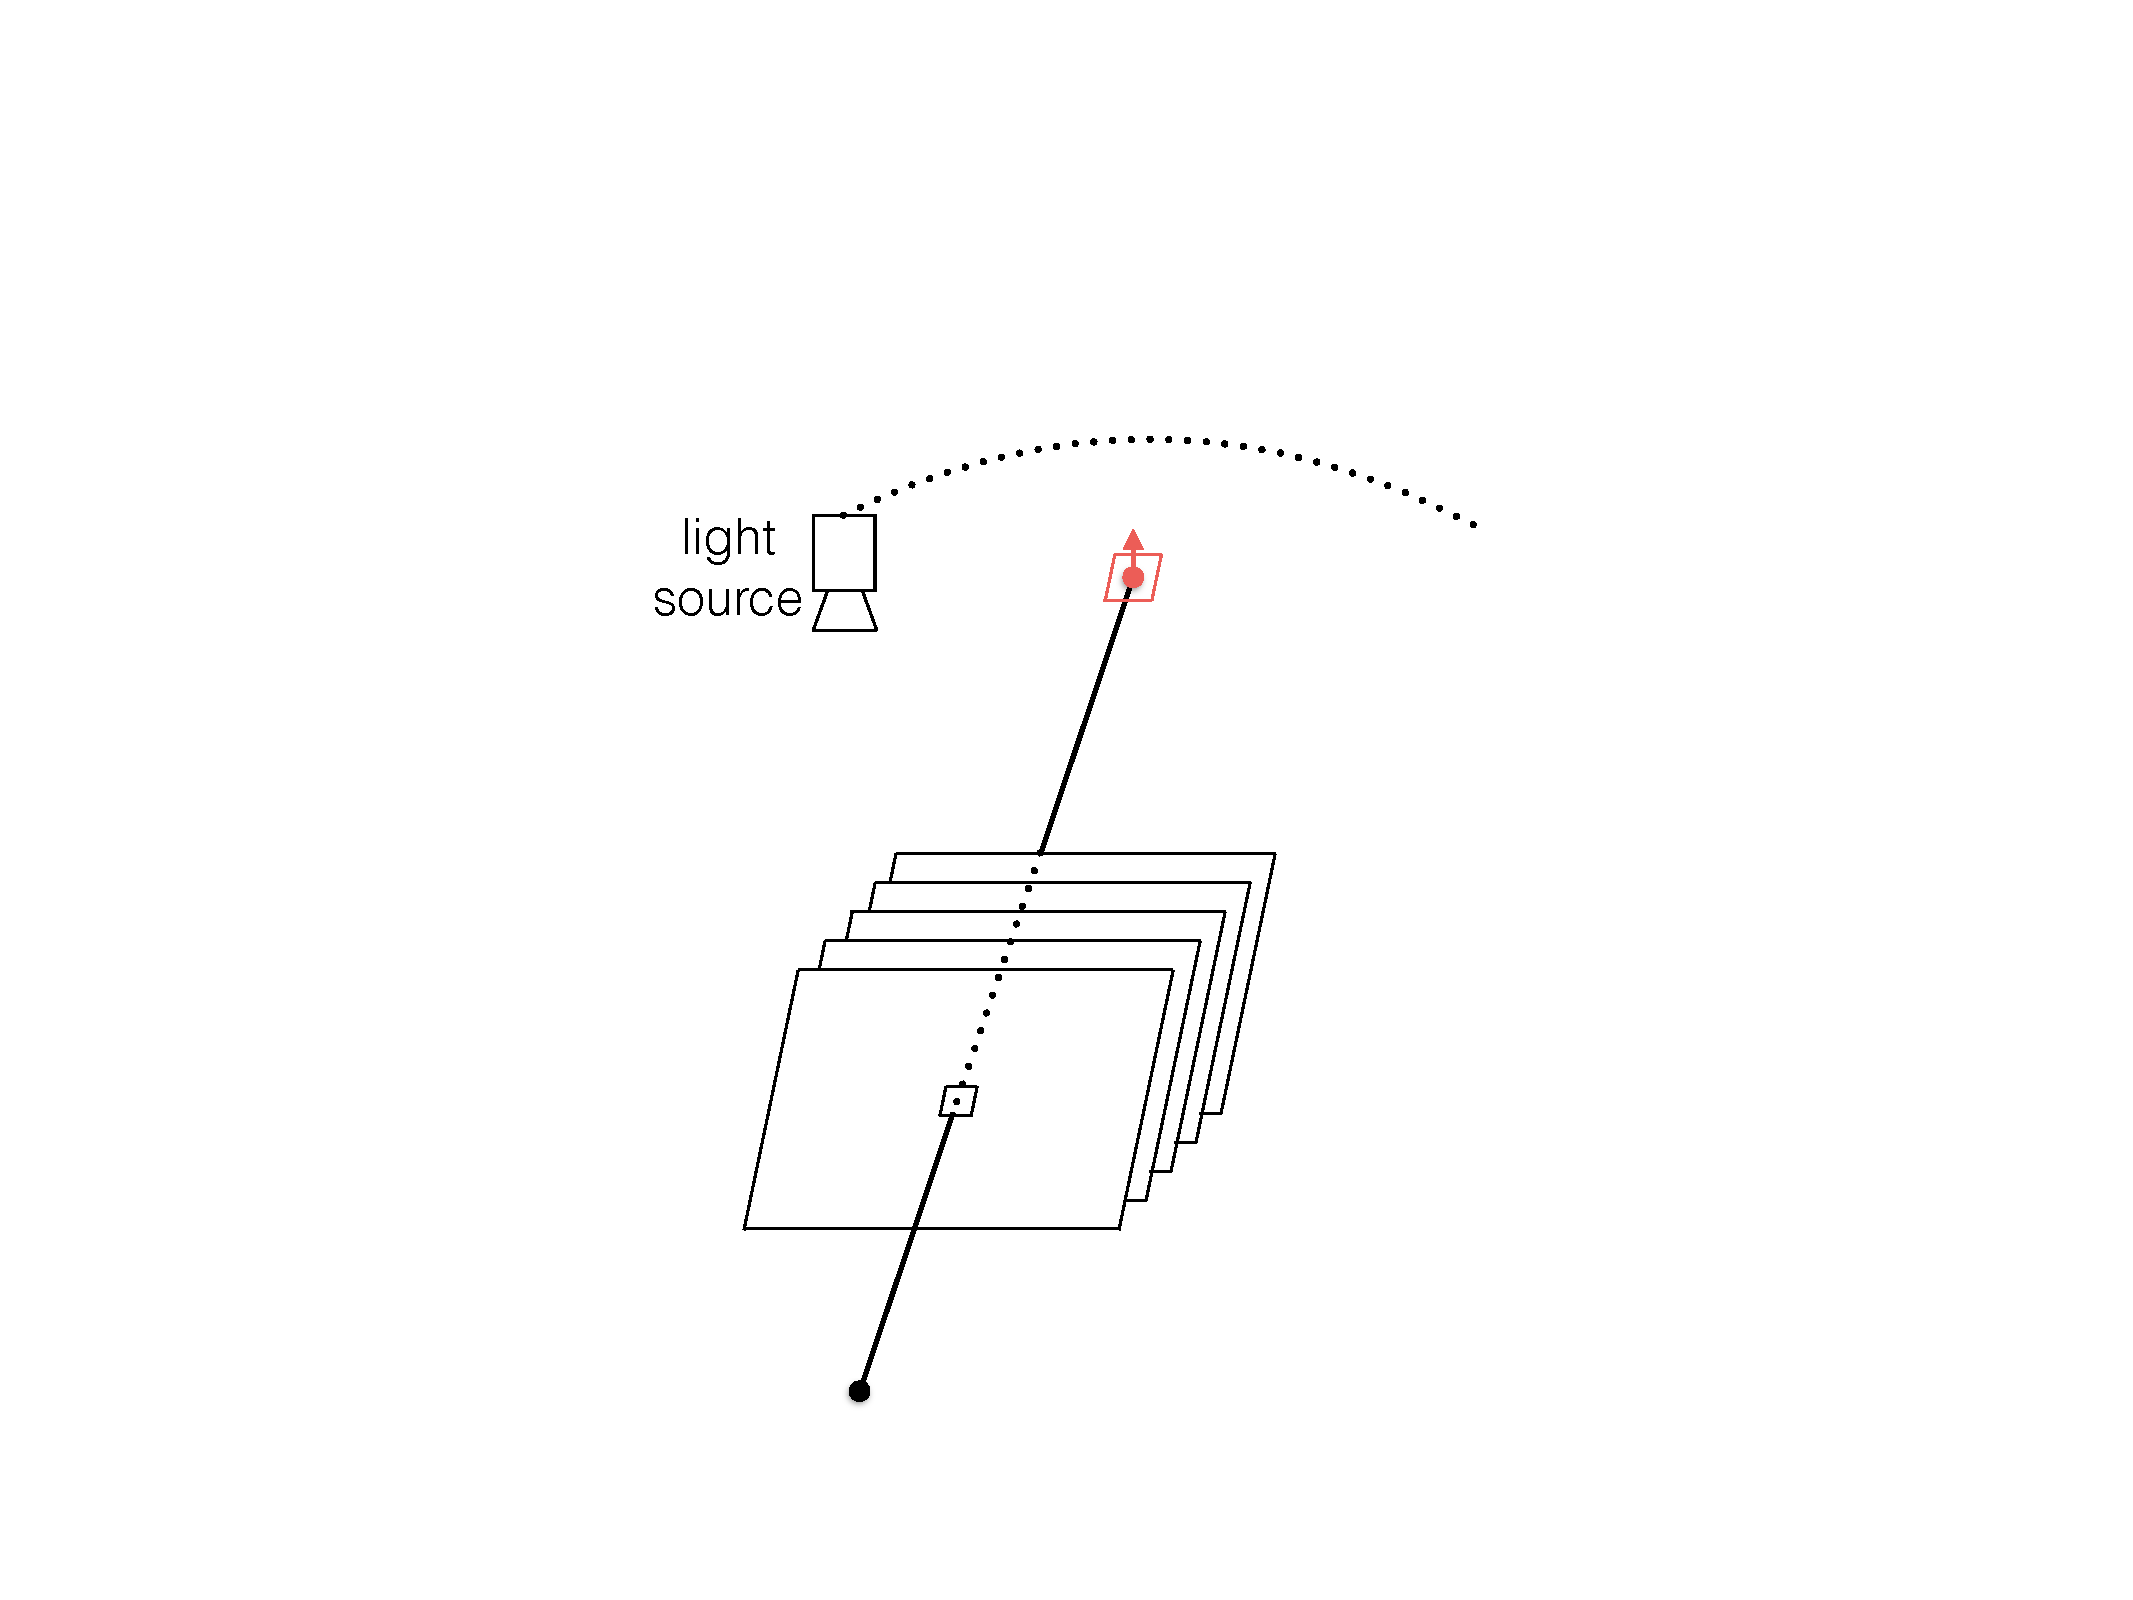
\includegraphics[width=0.5\texturewidth]{model/pixel_voxel}
% \caption{Pixel and voxel}
% \end{figure}

% \subsubsection{Silhouette and bounding edge}


% \subsubsection{Window area and patch}
% A window area is contained in a $w\times w$ regular square, and the surface patch is a 3D point of $p\times p$ with a normal vector.
% \begin{figure}[h]
% \centering
% 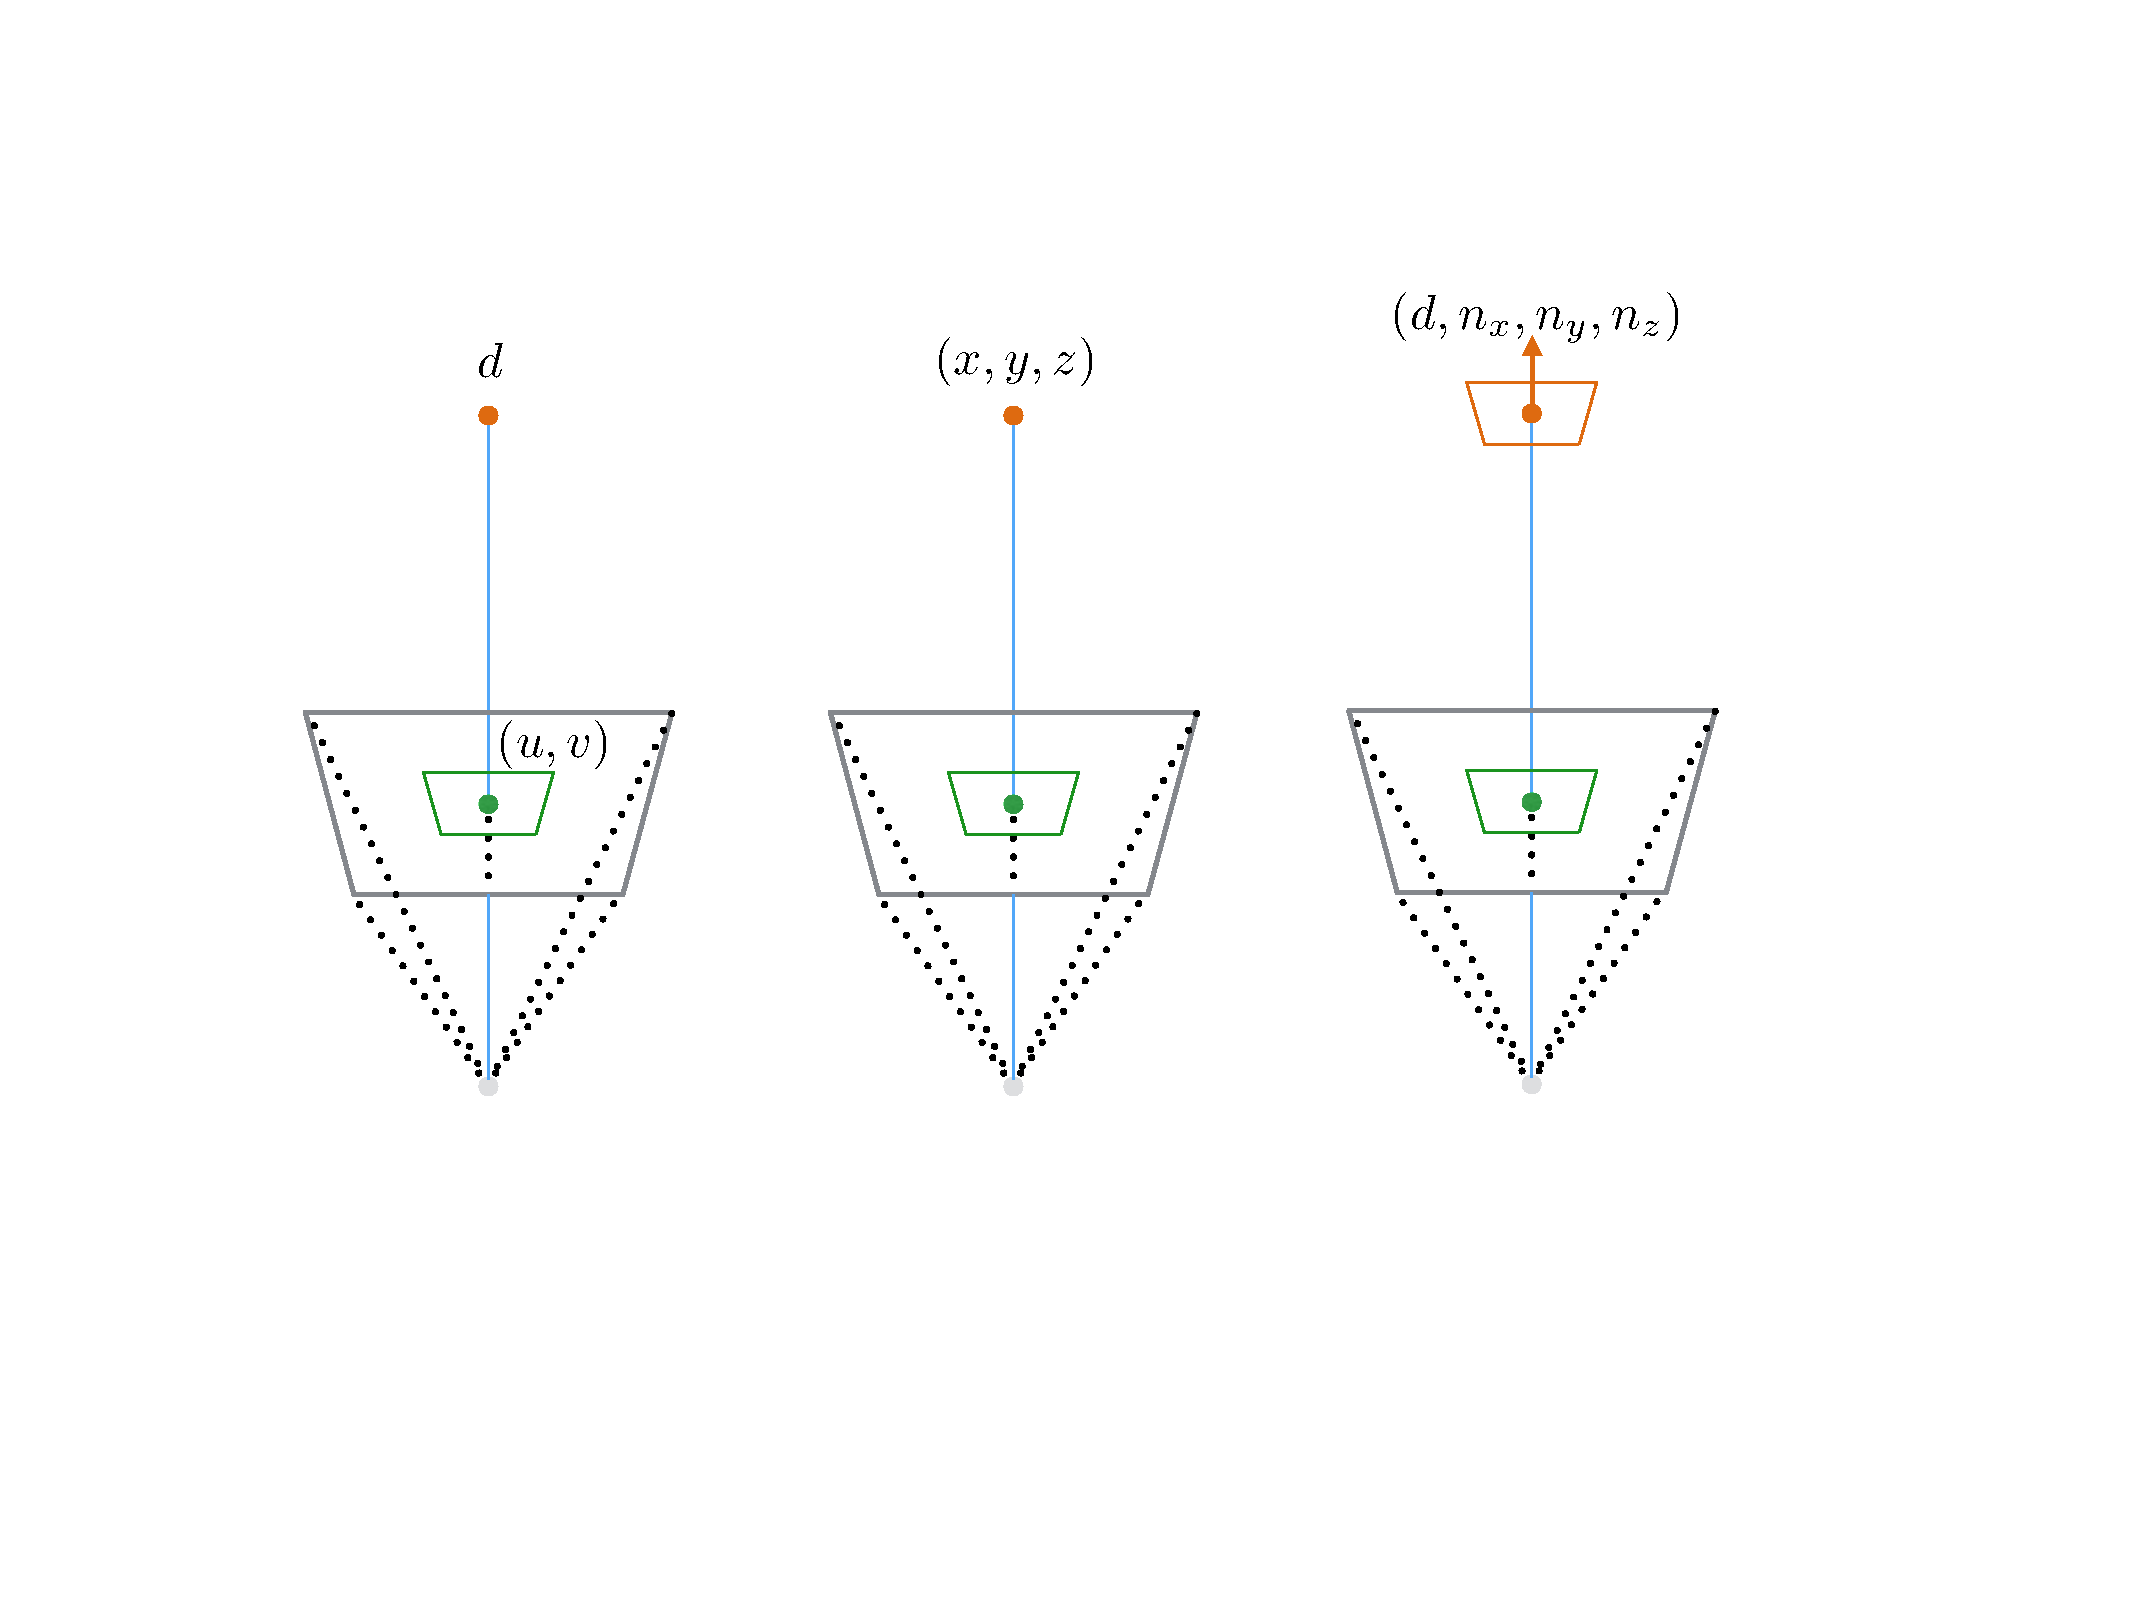
\includegraphics[width=0.8\textwidth]{model/window_patch}
% \caption{a window area and a surface patch}
% \end{figure}

% \subsection{Cues and properties}
% As defined in Chapter~\ref{sec:3DRecon_Def}, cue is the characteristics of the segment while property is that of the scell. For each cue observed in a segment, we discuss the underlying properties that have an impact on it.

\subsection{Texture}
Texture is one of the most important cues for many computer vision algorithms. It is generally divided into two categories, namely \textit{tactile} and \textit{visual} textures. Tactile textures refer to the immediate tangible feel of a surface whereas visual textures refer to the visual impression that textures produce to human observer, which are related to local spatial variations of simple stimuli like colour, orientation and intensity in an image. We focus only on visual textures as it's the most widely used ones in the stereo vision research, thus the term `texture' thereafter is exclusively referred to `visual texture' unless mentioned otherwise.

Although texture is an important component in computer vision, there is no precise definition of the notion texture. The main reason is that natural textures often exhibit different yet contradicting properties, such as regularity versus randomness, uniformity versus distortion, which can hardly be described in a unified manner. 
% Haralick considers a texture as an ``organized area phenomenon'' which can be decomposed into `primitives' having specific spatial distributions~\cite{haralick1979statistical}. This definition, also known as structural approach, comes directly from human visual experience of texture. These primitives are organized in a particular spatial structure indicating certain underlying placement rules. Alternatively, as Cross and Jain suggested, a texture is ``a stochastic, possibly periodic, two-dimensional image field''~\cite{cross1983markov}, which is also known as \textit{stochastic approach}.

% For s regular textures, there are two basic dimensions on which it may be described. The first dimension is for describing the primitives out of which the texture is composed, and the second dimension is for the description of the spatial dependence or interaction between the primitives of an image texture. The first property is concerned with tonal primitives and local properties, and the second dimension is concerned with the spatial organization of the tonal primitives.

There are various properties that make the texture distinguishable: scale/size/granularity, orientation, homogeneity, randomness, and etc. However, due to the diverse and complexity of natural textures, it's a challenging task to map from these semantic meanings to the precise properties of a synthetic texture. The stereo vision community often take a simplified approach, classifying them into two categories: regular and stochastic ones by their degree of randomness. A regular texture is formed by regular tiling of easily identifiable elements (texels) organized into strong periodic patterns. A stochastic texture exhibits less noticeable elements and display rather random patterns. Most of the real world texture are mixtures of these two categories. We adopt another simplification and consider \textit{texture coverage}, which is the ratio of the surface that is textured. Stereo vision, in theory, attempts to find the correspondences based on the `distinctiveness' of the texture. Therefore, as long as the surface is covered by distinctive texture, it make little difference what the basic building texture element is.

% Most texture synthetic research has focused on data-driven or statistical approaches. For the data-driven approach, the generated texture is not general enough whereas it's not intuitive enough for the statistical approach. Thus we turn to an approach that is more tailored to the stereo vision problem. Based on the observations from practical tests, stereo algorithms work well under the condition of non-uniform texture, even for textures caused by shadow. This is theoretically plausible as stereo vision tries to find the correspondence based on the `distinctiveness' of the texture. Therefore, as long as the surface is covered by distinct texture, it doesn't matter what the basic texture element is. Thus the most significant attributes of the texture is coverage, \ie the percent of the surface that is covered, and it's the focus of this thesis.

% Texture is formally defined as a set of texture element or \textit{texels} occuring in some regular, or repeated, or random pattern. Texture gives us information about the \textit{spatial arrangement} of the colours or intensities in an image. However, it is something that is easy to recognize, but hard to define. 

% Here we only consider visual textures, which is the result of shape and reflection. Therefore, a surface with varying reflectance property can produces a textured surface, a flat surface with fixed reflectance property under different illuminations can also achieve textured effect. Even very weak texture can be a strong cue to object reconstruction as manifested by the Middlebury `Dino' dataset.

\subsection{Lightness}
When light strikes a surface, it may be reflected, transmitted, absorbed, or scattered; usually, a combination of these effects occur. The intensity/colour information received by the sensor is thus determined, among other factors, the amount of light after these interaction. We consider intensity caused solely by reflection as it is the most common phenomenon and the easiest to analyse. Generally, we assume that all effects are local, thus global effects such as inter-reflection, transmission, and etc are omitted, which is called a \textbf{local interaction model}. Lightness ranges from `black' to `white' in the grey scale axis. Colour is a superset intensity, which takes account into the spectral composition of light. Both terms depend on illumination, surface normal, surface reflectance, and viewing direction.

In order to understand the contributing factor of pixel intensity/colour, we need a in-depth understanding of reflection, \ie how light is reflected off of a surface patch, and the relation between material and intensity value. The radiometric formation of an image consists of three separate process, \textit{light-matter interaction}, \textit{light-lens interaction}, and \textit{light-sensor interaction}.

\subsubsection{Definition of Radiometric Terms}
Here is a list of radiometry terms, see Figure~\ref{fig:radiometry_terms} for an illustration:
\begin{itemize}
\item Solid angle ($d\omega$): 3D counterpart of angle, $d\omega=\frac{dA \cos\theta_i}{R^2}\mathit{ (steradian)}$.
\item Projected solid angle ($d\Omega$): $d\Omega = \cos\theta d\omega$.
\item Incident radiance ($\mathbf{L_i(\theta_i, \phi_i)}$): light flux received from the direction $(\theta_i, \phi_i)$ on a unit surface area, unit $\mathit{ (watt\cdot m^{-2}\cdot steradian^{-1})}$.
\item Irradiance ($\mathbf{E_i(\theta_i, \phi_i)}$): light Flux (power) incident per unit surface area from all direction, $\mathbf{E_i(\theta_i, \phi_i)}=\int_{\Omega_i} L_i(\theta_i, \phi_i) d\Omega_i \mathit{ (watt/m^2)}$.
\item Surface radiance ($\mathbf{L_r(\theta_r, \phi_r)}$): light flux emmited from a unit surface area in the direction $(\theta_r, \phi_r)$, unit $\mathit{ (watt\cdot m^{-2}\cdot steradian^{-1})}$.
\end{itemize}

\begin{figure}[!ht]
\centering
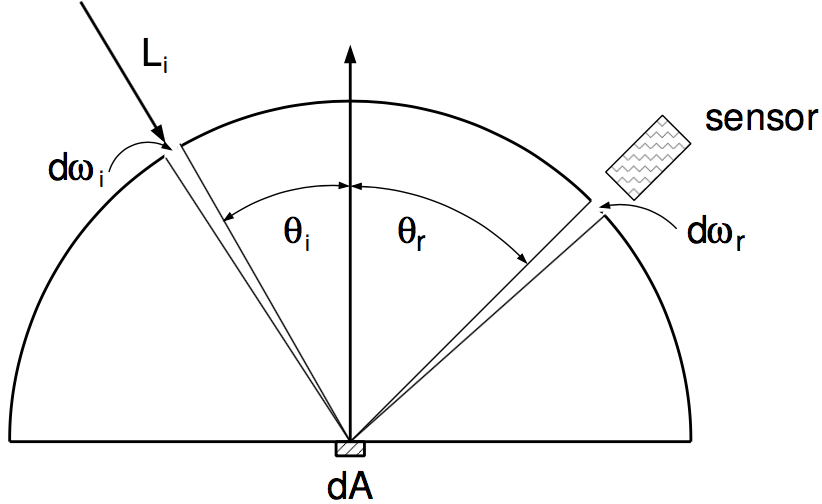
\includegraphics[width=0.5\textwidth]{model/radiometry_terms.png}
\caption{Light-matter interaction}
\label{fig:radiometry_terms}
\end{figure}

\subsubsection{Light-matter interaction}
The relation between the incoming illumination and reflected light is model using the \textit{bidirectional reflectance distribution function}, usually abbreviated BRDF. The BRDF is define as

\textbf{Definition (BRDF)} the ratio of the surface radiance $\mathbf{L_r(\theta_r, \phi_r)}$ to the irradiance $\mathbf{E_i(\theta_i, \phi_i)}$, \ie $f(\theta_i, \phi_i, \theta_r, \phi_r)=\frac{E^{surface}(\theta_i, \phi_i)}{L^{surface}(\theta_r, \phi_r)}$.

\begin{figure}[!ht]
\centering
\begin{tikzpicture}[node distance=2cm, auto]
\node (light) [model_nonfixed] {Light};
\node (brdf) [process_nonfixed, inner sep=0pt, right of=light, xshift=1cm] {BRDF};
\node (scene) [model_nonfixed, right of=brdf, xshift=1cm] {Scene};
\node (scene_rad) [data_nonfixed, right of=scene, xshift=1cm] {Scene Radiance};
\draw [arrow] (light) -- (brdf);
\draw [arrow] (brdf) -- (scene);
\draw [arrow] (scene) -- (scene_rad);
\end{tikzpicture}
\caption{The light-matter interaction.}
\label{fig:light_matter_interact}
\end{figure}

\textbf{Diffuse Albedo} or surface lightness is the proportion of incident light that is reflected by the surface. It should be noted that albedo is not an intrinsic property of a surface. Instead, for any surface, the albedo depends on the spectral and angular distributions of the incident light.

\subsubsection{Light lens interaction}
The assumption made in vision is that radiance is constant as it propagates along ray. Therefore the scene radiance is the same as the radiance hitting on the camera sensor. It can be further shown that the image irradiance received by the sensor is proportional to the scene radiance, thus the relation between \textit{scene radiance} and \textit{image irradiance} is linear.
\begin{figure}[!ht]
\centering
\begin{tikzpicture}[node distance=2cm, auto]
\node (scene_rad) [data] {Scene Radiance};
\node (lens) [model, right of=scene_rad, xshift=2cm] {Lens};
\node (irradiance) [data, right of=lens, xshift=2cm] {Image Irradiance};
\draw [arrow] (scene_rad) -- (lens);
\draw [arrow] (lens) -- (irradiance);
\end{tikzpicture}
\caption{The light-lens interaction.}
\label{fig:light_lens_interact}
\end{figure}

\subsubsection{Light sensor interaction}
The camera response function relating image irradiance at the image plane to the measured pixel intensity values is a non-linear mapping. A linear relation can be retrieved by radiometric calibration.
\begin{figure}[!ht]
\centering
\begin{tikzpicture}[node distance=2cm, auto]
\node (irradiance) [data] {Image Irradiance};
\node (sensor) [model, right of=irradiance, xshift=2cm] {Sensor};
\node (intensity) [data, right of=sensor, xshift=2cm] {Intensity};
\draw [arrow] (irradiance) -- (sensor);
\draw [arrow] (sensor) -- (intensity);
\end{tikzpicture}
\caption{The light-sensor interaction.}
\label{fig:light_sensor_interact}
\end{figure}

In conclusion, if \textit{light sensor} is assumed as a linear mapping as most of vision algorithms do, or calibrated as a pre-processing step. The factor that influence the intensity is the BRDF value. There are 4 DoF for spatially-invariant BRDF, and for a special, simple case - Lambertian reflectance, the BRDF is degenerated to the diffuse \textit{albedo}, which is the representation we adopt for intensity.

% The reflectance of light also depends on the incident direction. Specifically, light that lands on a surface at a grazing angle will be much more likely to reflect, see Figure~\ref{fig:alb_ang}. We take into account the Fresnel effect in the synthetic stage, thus we consider the albedo with small incident angle.
% \begin{figure}[h]
% \centering
% 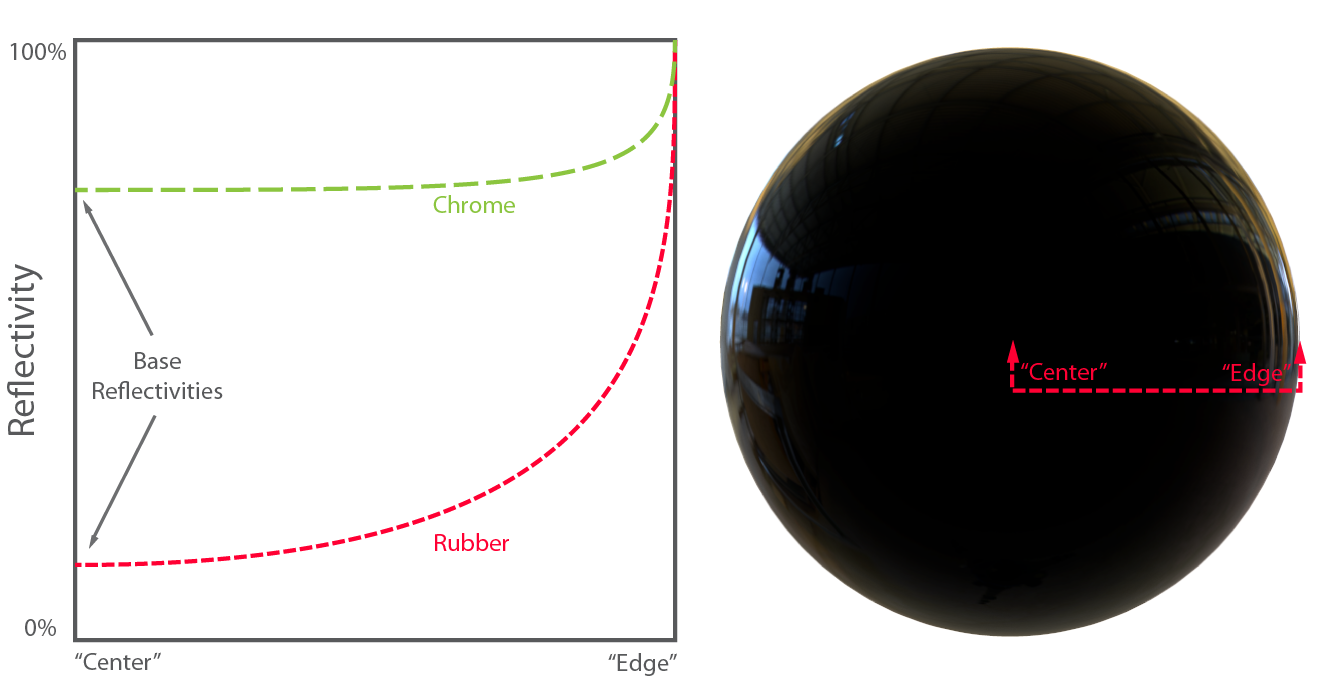
\includegraphics[width=0.5\textwidth]{model/reflectance_angle}
% \label{fig:alb_ang}
% % \caption{Spectral reflectance curves for aluminium (Al), silver (Ag), and gold (Au) metal mirrors at normal incidence.}
% \end{figure}

\subsection{Reflectance}
Specular surfaces reflect light in almost a single direction when the microscopic surface irregularities is small compared to light wavelength, and no subsurface scattering present~\cite{nayar1989surface}. Unlike diffuse reflections, which we experience the lightness and colour of an object, specular reflections carry information about the structure, intensity, and spectral content of the illumination field. In other words, specular reflection is simply image of the environment, or the illumination field, distorted by the geometry of the reflecting surface. See Figure~\ref{fig:spec_ref}, the image no long reflect the original colour of the surface (red), instead it shows a distorted image of the environment. A purely specular surface is a mirror. Purely specular surfaces are rare in nature. Most natural materials exhibit a mix of specular and diffuse reflection. Variations in microscopic surface geometry can cause specular reflections to be scattered, blurring the image of the environment in an amount proportional to surface roughness. We use a numeric \textit{specular}ps value to denote the proportion of specularity of the material, with 0 being completely diffuse, and 1 being completely specular or mirror light.
\begin{figure}[h]
\centering
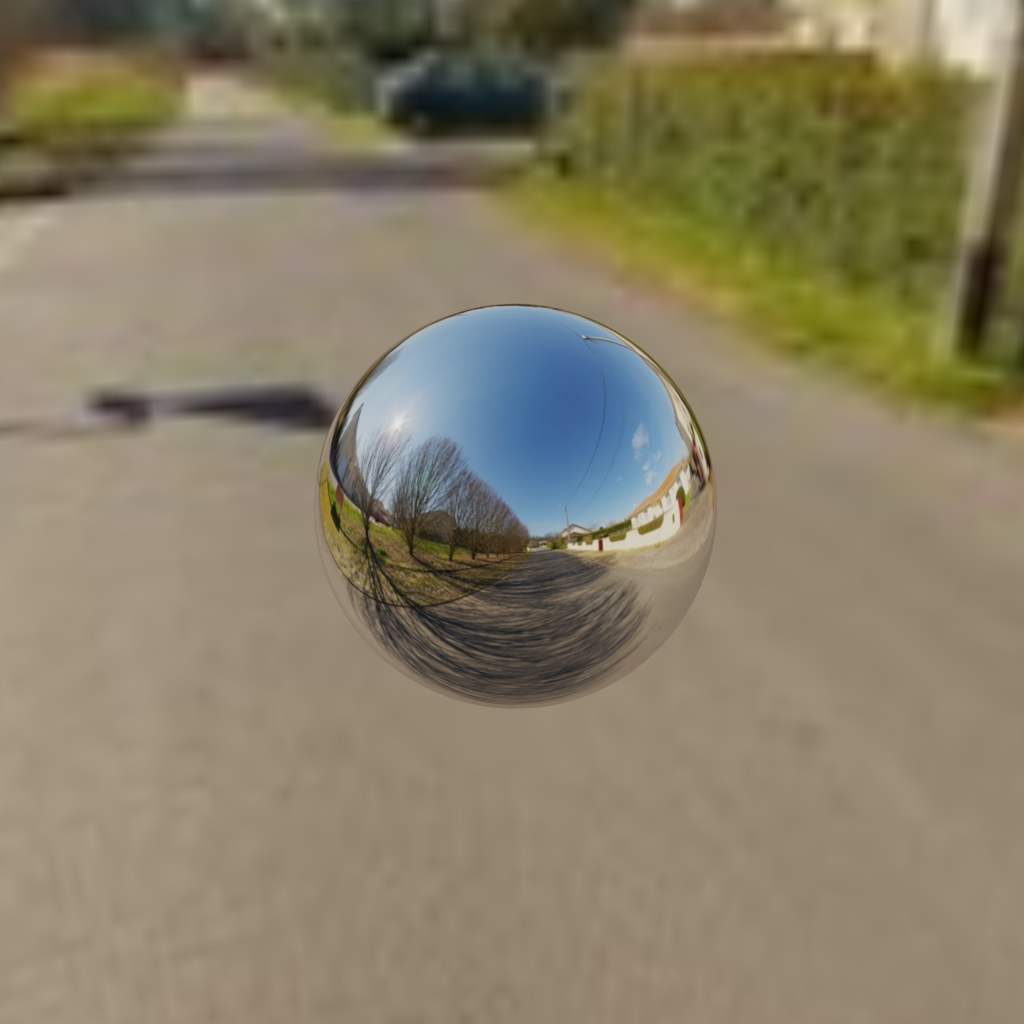
\includegraphics[width=0.5\textwidth]{model/spec_ref}
\caption{A \textbf{red} specular sphere. The surface reflects light in a mirror-like way, and no diffuse reflection exist, thus the colour of the surface is no longer visible.}
\label{fig:spec_ref}
\end{figure}

\subsection{Roughness}
Roughness, which is characterized as the microscopic shape characteristics of the surface, contributes to the way in which light is reflected off of a surface. A smooth surface may reflect incident light in a single direction, while a rough surface may scatter the light in various directions. We need prior knowledge of the microscopic surface irregularities, or a model of the surface to determine the reflection of incident light.

The possible surface models are divided into 2 categories: surface with exactly known profiles and surfaces with random irregularities. An exact profile may be determined by measuring the height at each point on the surface by means of a sensor such as the stylus profilometer. This method is cumbersome and impractical. Hence, it’s more reasonable to model the surface as a random process, where it is described by a statistical distribution of either its height above a certain mean level, or its slope w.r.t its mean (macroscopic) slope. The section only discusses these second statistical approach.

% \textit{Height Distribution Model} The height coordinate of the surface is expressed as random function of the coordinates $x$ and $y$.
% \begin{figure}[h]
% \centering
% \includegraphics[width=0.5\textwidth]{model/surface_representation_1}
% \caption{Surface height distribution model}
% \end{figure}

% The shape of the surface is determined by the probability distribution of $h$. For instance, let $h$ be normally distributed, with mean value $\bar{h}=0$ and standard deviation $\sigma_h$. Then, the distribution of $h$ is given by:
% $$
% p_h(h)=\frac{1}{\sqrt{2\pi}\sigma_h}e^{-\frac{h^2}{2\sigma_h^2}}
% $$

% The $\sigma_h$ is the root-mean-square of $h$ and represents the roughness of the surface. The surface is not uniquely described by the distribution of $h$, as it does not tell us anything about the distance between the hills and valleys of the surface.

% The surfaces below have the same height distribution function, i.e., the same mean value and standard deviation. However, they don't resemble each other in appearance.
% \begin{figure}[h]
% \centering
% \includegraphics[width=8cm]{model/same_mean_sd}
% \caption{Surface height distribution model}
% \end{figure}

% An autocorrelation coefficient $C(\tau)$ is introduced, that determines the correlation (or lack of independence) between the random values assumed by the height $h$ at two surface points $(x_1, y_1)$ and $(x_2, y_2)$, separated by a distance $\tau$. The autocorrelation coefficient can be:
% $$
% C(\tau)=e^{-\frac{\tau^2}{T^2}}
% $$

% where $T$ is the *correlation distance*. Therefore, the above surfaces have small and large correlation distances respectively.

\subsubsection{Slope Distribution Model}
We can think of a surface as a collection of planar micro-facets.
\begin{figure}[h]
\centering
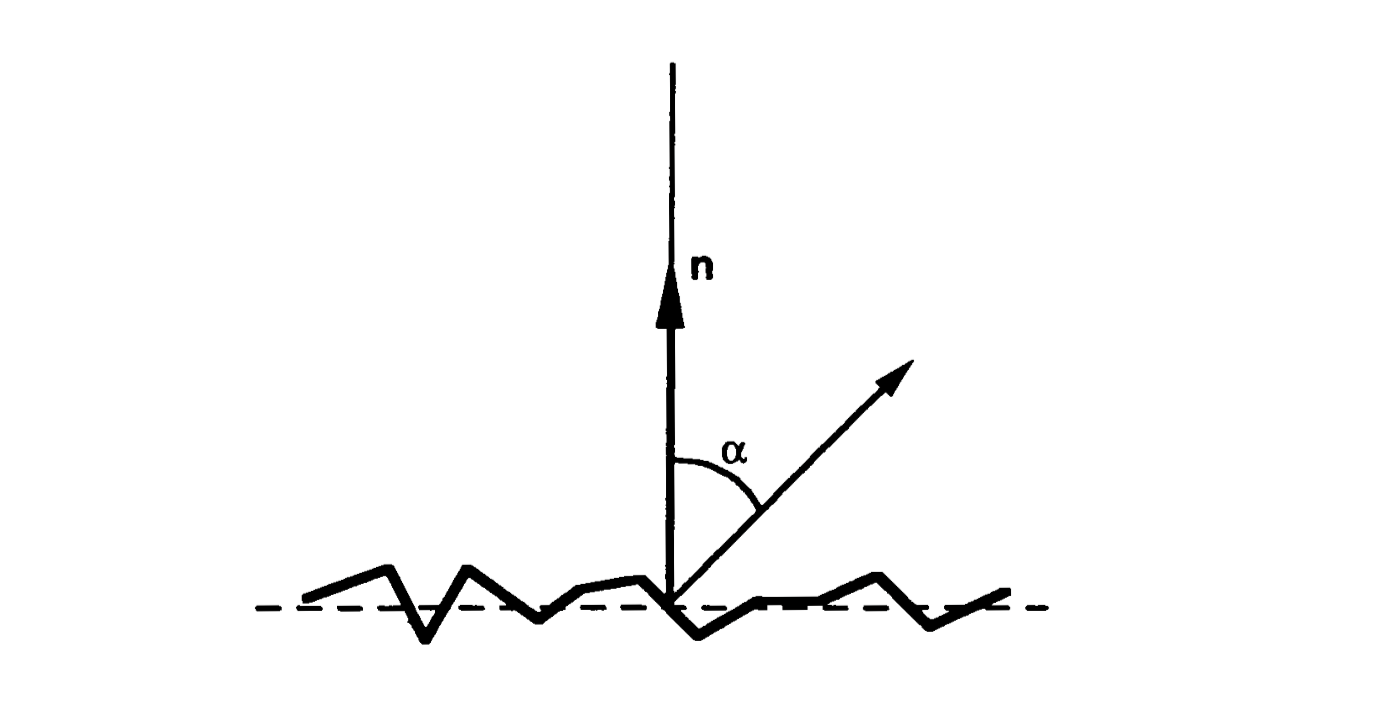
\includegraphics[width=0.7\textwidth]{model/surface_representation_2}
\caption{Surface Slope Distribution Model}
\end{figure}

A large set of micro-facets constitutes an infinitesimal surface patch that has a mean surface orientation $\vec{n}$. Each micro-facet has its own orientation, which may deviate from the mean surface orientation by an angle $\alpha$.

We will use the parameter $\alpha$ to represent the slope of individual facets. Surfaces can be modeled by a statistical distribution of the micro-facet slopes. If the surface is isotropic, the probability distribution of the micro-facet slopes can be assumed to be rotationally symmetric w.r.t the mean surface normal $\vec{n}$.  Therefore, facet slopes can be described by a one-dimensional probability distribution function. For instance, the surface may be modeled by assuming a normal distribution for the facet slope $\alpha$, with mean value $\bar{\alpha}=0$ and standard deviation $\sigma_\alpha$, and larger $\sigma_\alpha$ can be used to model rougher surfaces:
$$
p_\alpha(\alpha)=\frac{1}{\sqrt{2\pi}\sigma_\alpha}e^{-\frac{\alpha^2}{2\sigma_\alpha^2}}
$$

% The surface model is determined by a single parameter $\sigma_\alpha$ While autocorrelation coefficient is important, the concept of slope correlation is more difficult to interpret and is not that useful in the generation of surface, which results in a weaker model compared to the height model. However, slope distribution model is popular in the analysis of surface reflection, as the scattering of light rays is dependent on the local slope of the surface and not the local height of the surface.

% surface roughness will affect the fresnel and specularity

\subsection{Concavity}
Concavity can cause self-shadow or inter-reflection effect, which can severely impede the accuracy of intensity based algorithms. Since concavity is not shown in the silhouette image, methods that utilize silhouette information may also fail to reconstruct concavities. Concavity is measured by \textit{surface curvature}.

% \subsubsection{Silhouette}
% \textbf{Concavity} is not shown in the silhouette image, thus methods that utilize silhouette information may fail to reconstruct concavities. Concavity is measured by \textit{surface curvature}.

\section{Expression}
\label{sec:3DRecon_Exp}
Now with the proposed definition and representation of 3D reconstruction problem, we can express some existing 3D reconstruction algorithms under this framework. The expression of the reconstruction problem is shown in table~\ref{tab:express}.
\begin{table}[h]
  \centering
  \begin{tabular}{l*{5}{c}}
  \hline
  \textbf{object} & Texture coverage & Albedo & Specular & Roughness & Concavity\\
  \hline
  Class 1 & 0.2 & 0.8 & 0.2 & 0.8 & 0.2\\
  Class 2 & 0.2 & 0.8 & 0.5 & 0.2 & 0.2\\
  Class 3 & 0.8 & 0.8 & 0.2 & 0.8 & 0.2\\
  Class 5 & 0.8 & 0.8 & 0.5 & 0.2 & 0.2\\
  \hline
  \end{tabular}
  \caption{Expression of the reconstruction problem for the object class 1, 2, 3, 5.}
  \label{tab:express}
\end{table}